\documentclass{article}
\usepackage[utf8]{inputenc}
\usepackage[polish]{babel}
\usepackage[T1]{fontenc}
\usepackage{graphicx}
\usepackage{float}
\usepackage[a4paper, left=3.7cm, right=3.7cm, top=3cm, bottom=2cm]{geometry}

\title{Projekt PAM - aplikacja służąca do rozwiązywania testów}
\author{Antoni Załupka}

\begin{document}
	\thispagestyle{empty}
	
	
	\vspace{4cm}
	
	\rule{\linewidth}{2mm} 
	
	\begin{center}
		\huge \textbf{Projektowanie Webowych Aplikacji Graficznych} \\
		\huge {Aplikacja webowa służąca do rozwiązywania testów} \\
	\end{center}
	
	\rule{\linewidth}{0.5mm} 
	
	\vspace{2cm}
	
	\begin{center}
		\Large{Antoni Załupka} \\
		\Large{Numer indeksu: 351120} \\
		\Large{III rok, grupa PAW2} \\
		
	\end{center}
	
	
	\vspace{15cm}
	
	\begin{center}
		\Large{2025, Uniwersytet Śląski}
	\end{center}
	
	\newpage
	
	\section{Wstęp}
	Celem niniejszego projektu było zaprojektowanie oraz zaimplementowanie edukacyjnej aplikacji webowej w formie quizów stworzonej z wykorzystaniem technologii Vue. Aplikacja ma też uproszczoną wersję mobilną. 
	
	Quizy dostępne w aplikacji nie służą wyłącznie weryfikacji wiedzy użytkownika, lecz pełnią funkcję edukacyjną. Każde pytanie umożliwia niezwłoczne sprawdzenie poprawności odpowiedzi oraz jej modyfikację, co umożliwia naukę w oparciu o szybką informację zwrotną.

    \section{Założenia}
    \subsection*{Wymagania funkcjonalne}
	\begin{itemize}
		\item Możliwość logowania do aplikacji;
		\item Pobieranie danych z API, w tym quizów oraz historii podejść użytkownika;
		\item Rozwiązywanie quizów i natychmiastowe, asynchroniczne zapisywanie postępu;
		\item Przeglądanie historii podejść w dedykowanej zakładce;
		\item Możliwość edycji, usunięcia i wylogowania się z konta.
	\end{itemize}
	
	\subsection*{Wymagania niefunkcjonalne}
	\begin{itemize}
		\item Intuicyjny i przejrzysty interfejs użytkownika;
		\item Wysoka responsywność aplikacji na różnych urządzeniach;
		\item Bezpieczna obsługa danych użytkownika (autoryzacja poprzez token JWT);
		\item Wydajna komunikacja z API (minimalizacja liczby zapytań);
		\item Utrzymanie spójności z wersją mobilną aplikacji.
	\end{itemize}

    \section{Kontekst}
        Aplikacja została stworzona symultanicznie z wersją mobilną. 
        Wersja mobilna jest uproszczona i została napisana w technologii Flutter.
        Obie aplikacje korzystają z tego samego API. 
        API wykonałem w technologii GraphQL, co pozwoliło na elastyczne pobieranie danych i minimalizację liczby zapytań.
        Obie części napisałem w języku TypeScript, co zapewniło lepszą kontrolę typów i ułatwiło rozwój projektu.
        W dalszej części sprawozdania skupię się na webowej części projektu.

    \section{Wykorzystane technologie}
        Backend:
        \begin{itemize}
            \item Interpreter JavaScript Node.js
            \item Framework Express
            \item Komunikacja GraphQL
            \item Baza danych SQLite
        \end{itemize}
        Frontend:
        \begin{itemize}
            \item Vite - szybki bundler i serwer deweloperski
            \item Vue.js - framework do budowy interfejsu
            \item Pinia - zarządzanie stanem aplikacji
            \item Shadcn - biblioteka komponentów UI
            \item Apollo Client - komunikacja z API GraphQL
            \item Vue Router - zarządzanie trasami aplikacji
            \item Tailwind CSS - framework CSS do stylizacji za pomocą klas
        \end{itemize}

    \section{Struktura projektu}
    \begin{itemize}
      \item \textbf{frontend/}
      \begin{itemize}
        \item \textbf{public/}
        \begin{itemize}
          \item \textbf{index.html} – główny plik HTML aplikacji
        \end{itemize}
        \item \textbf{src/}
        \begin{itemize}
          \item \textbf{main.ts} – punkt wejścia Vue, inicjalizacja Pinia i routera
          \item \textbf{App.vue} – główny komponent aplikacji
          \item \textbf{router.ts} – konfiguracja tras (vue-router)
          \item \textbf{apollo-client.ts} – konfiguracja klienta GraphQL (Apollo)
          \item \textbf{style.css} – globalne style CSS i zmienne koloru
          \item \textbf{vite.config.ts} – konfiguracja bundlera i serwera deweloperskiego (Vite)
          \item \textbf{vite-env.d.ts} – definicje typów dla Vite
          \item \textbf{components/} – komponenty UI (ui/, Header/, itp.)
          \item \textbf{pages/} – widoki i strony routowane
          \item \textbf{stores/} – magazyny stanów (Pinia: userStore, attemptStore)
          \item \textbf{services/} – usługi komunikacji z API (quizService, aiService, itp.)
          \item \textbf{lib/} – funkcje pomocnicze (utils.ts)
        \end{itemize}
        \item \textbf{package.json}, \textbf{tsconfig.json}, \textbf{README.md}
      \end{itemize}
    \end{itemize}

    \section{Wdrożenie aplikacji}

        Aplikację wdrożyłem na własnym serwerze VPS, używając Nginx jako serwera proxy. Frontend jest dostępny pod adresem \texttt{https://quiz.azalupka.cc}. Aplikacja została zbudowana przy użyciu Vite, co pozwoliło na optymalizację rozmiaru paczek oraz czasu ładowania. Do przygotowania i lokalnego sprawdzenia wersji produkcyjnej wykorzystałem następujące polecenia:

        \begin{verbatim}
            npm run build
            npm run preview
        \end{verbatim}

    \section{Galeria efektów końcowych}
      \begin{enumerate}

        \item Strona główna \\
        \begin{minipage}{0.4\textwidth}
          \begin{itemize}
            \item Po uruchomieniu aplikacji wyświetla się widok zachęcający użytkownika do zalogowania lub rejestracji.
          \end{itemize}
        \end{minipage}
        \begin{minipage}{0.6\textwidth}
          \begin{figure}[H]
            \centering
            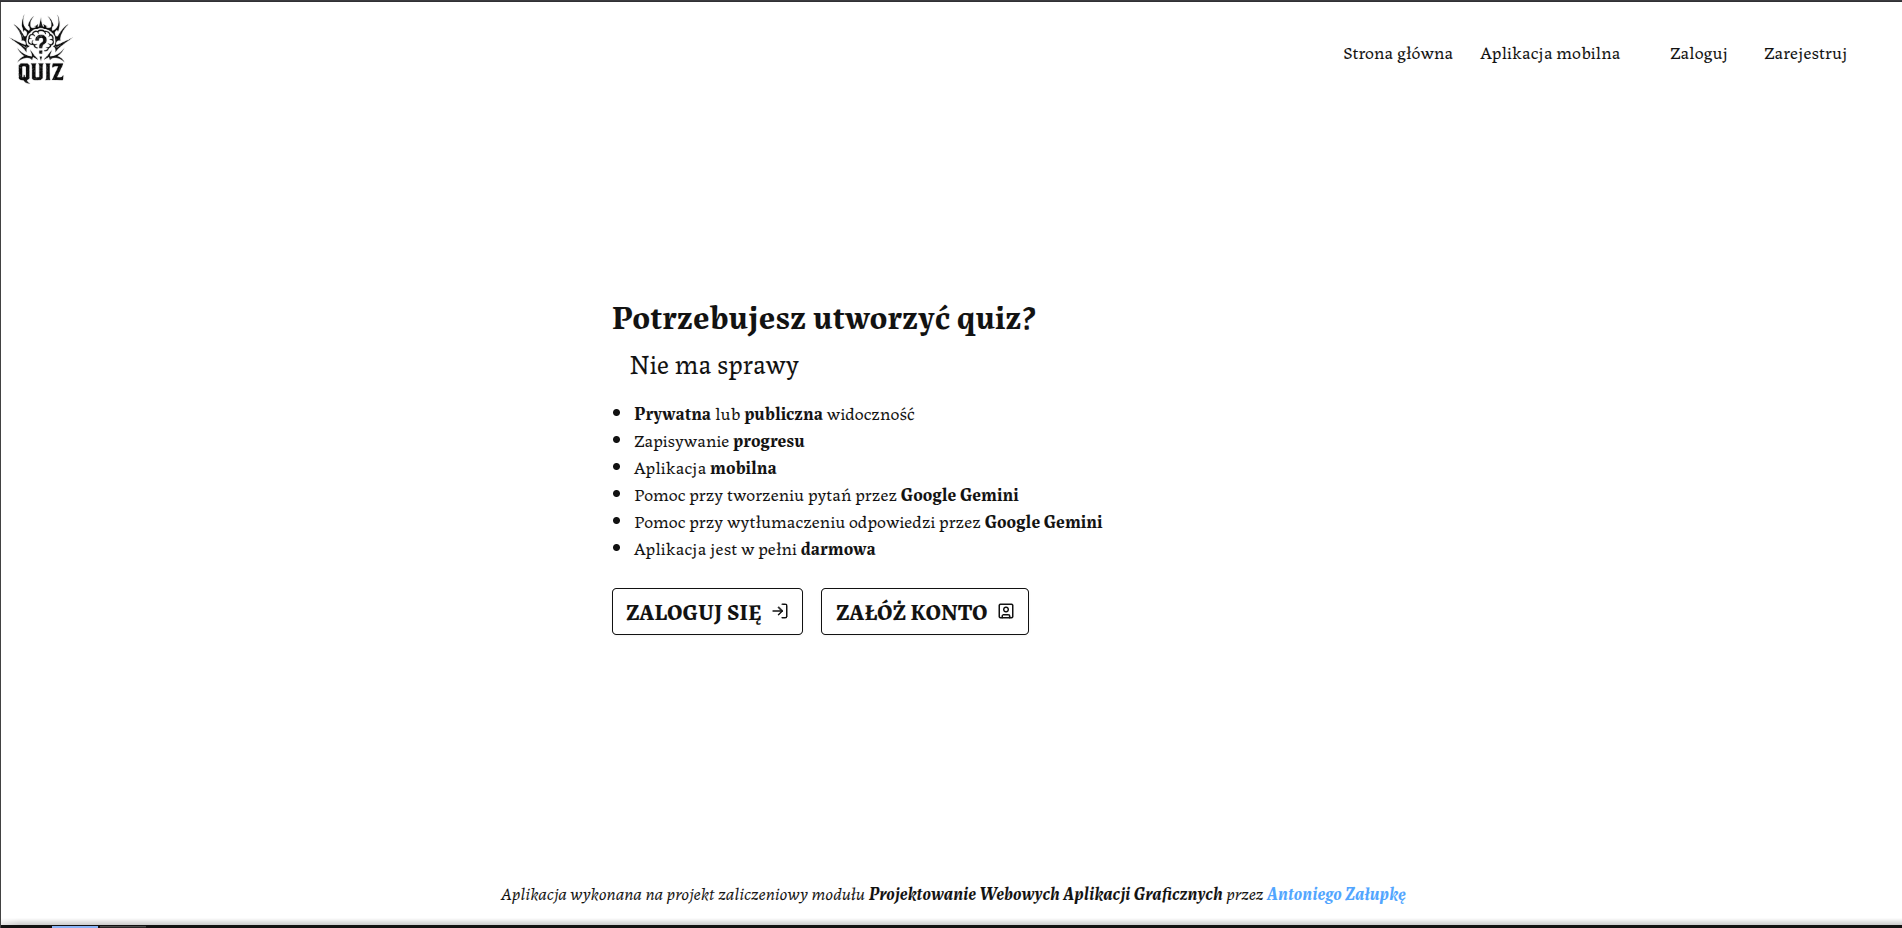
\includegraphics[width=0.5\textwidth]{../_assets/web/index.png}
            \caption{Strona główna przed zalogowaniem.}
            \label{fig:index}
          \end{figure}
        \end{minipage}

        \item Kreator quizu \\
        \begin{minipage}{0.4\textwidth}
          \begin{itemize}
            \item Możemy wygenerować quiz za pomocą modelu językowego Google Gemini.
          \end{itemize}
        \end{minipage}
        \begin{minipage}{0.6\textwidth}
          \begin{figure}[H]
            \centering
            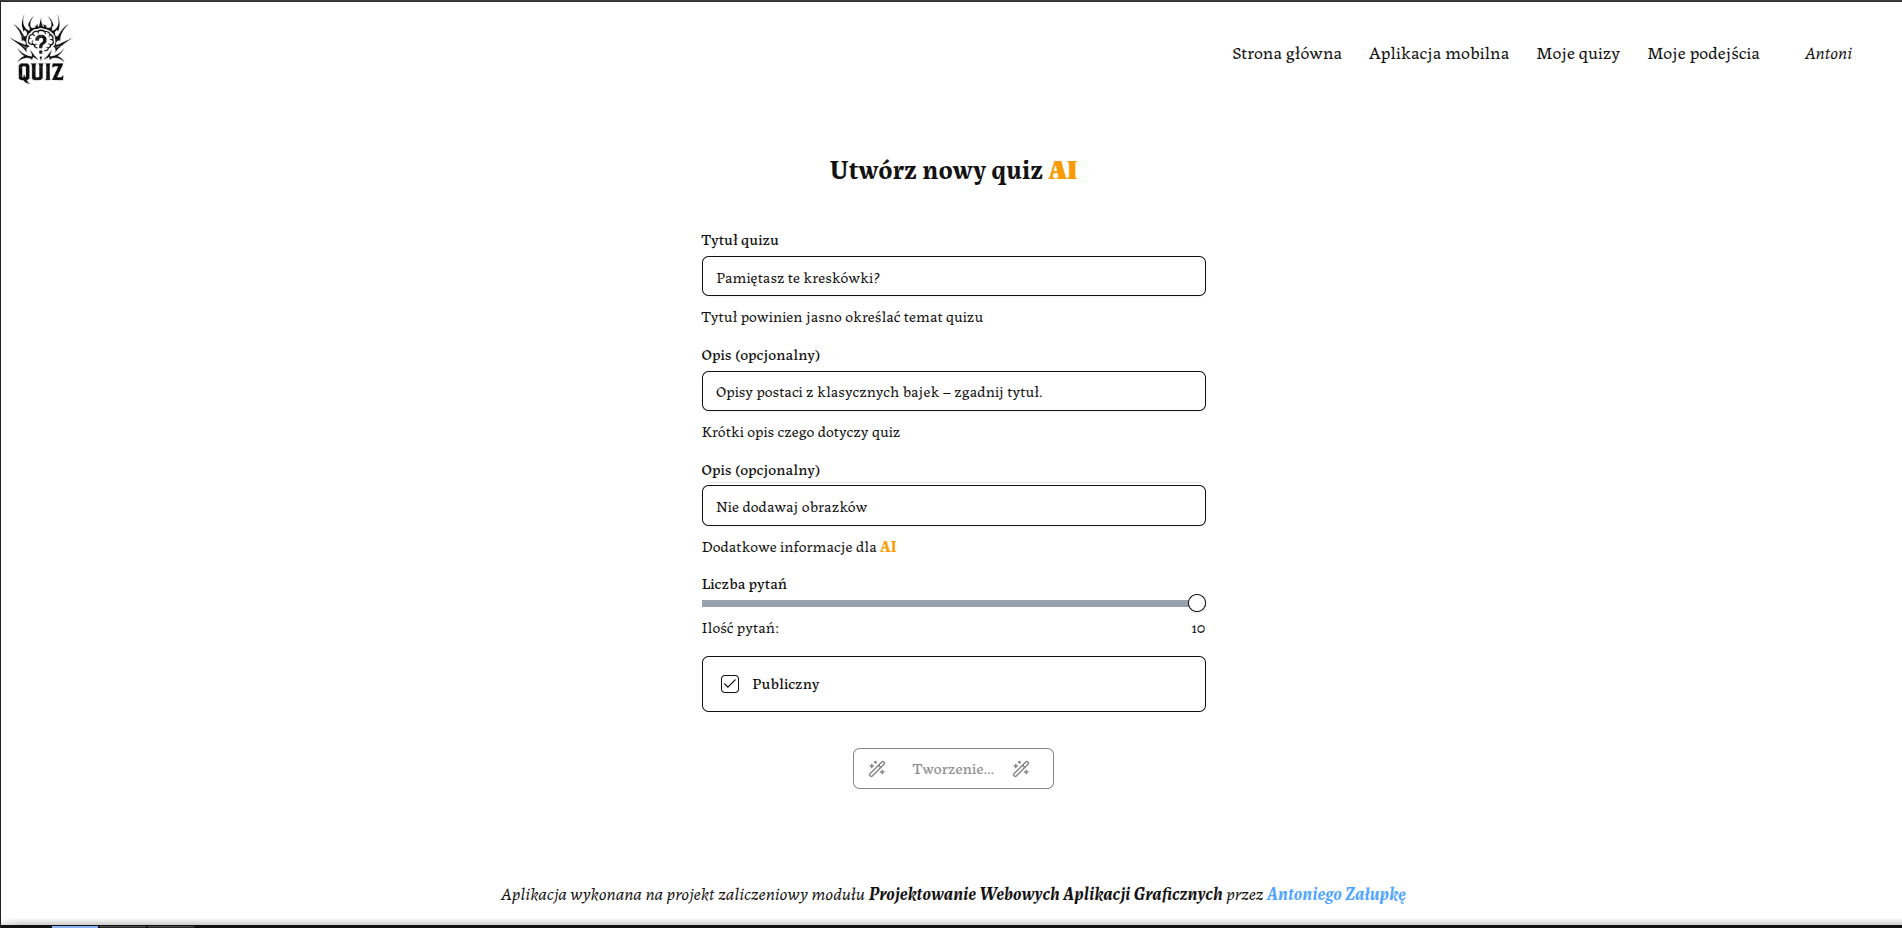
\includegraphics[width=0.5\textwidth]{../_assets/web/createAi.png}
            \caption{Automatyczny kreator tworzenia quizu.}
            \label{fig:createAi}
          \end{figure}
        \end{minipage}

		\item Edytor quizu \\
        \begin{minipage}{0.4\textwidth}
          \begin{itemize}
            \item Quiz możemy również stworzyć lub edytować ręcznie, korzystając z edytora JSON.
          \end{itemize}
        \end{minipage}
        \begin{minipage}{0.6\textwidth}
          \begin{figure}[H]
            \centering
            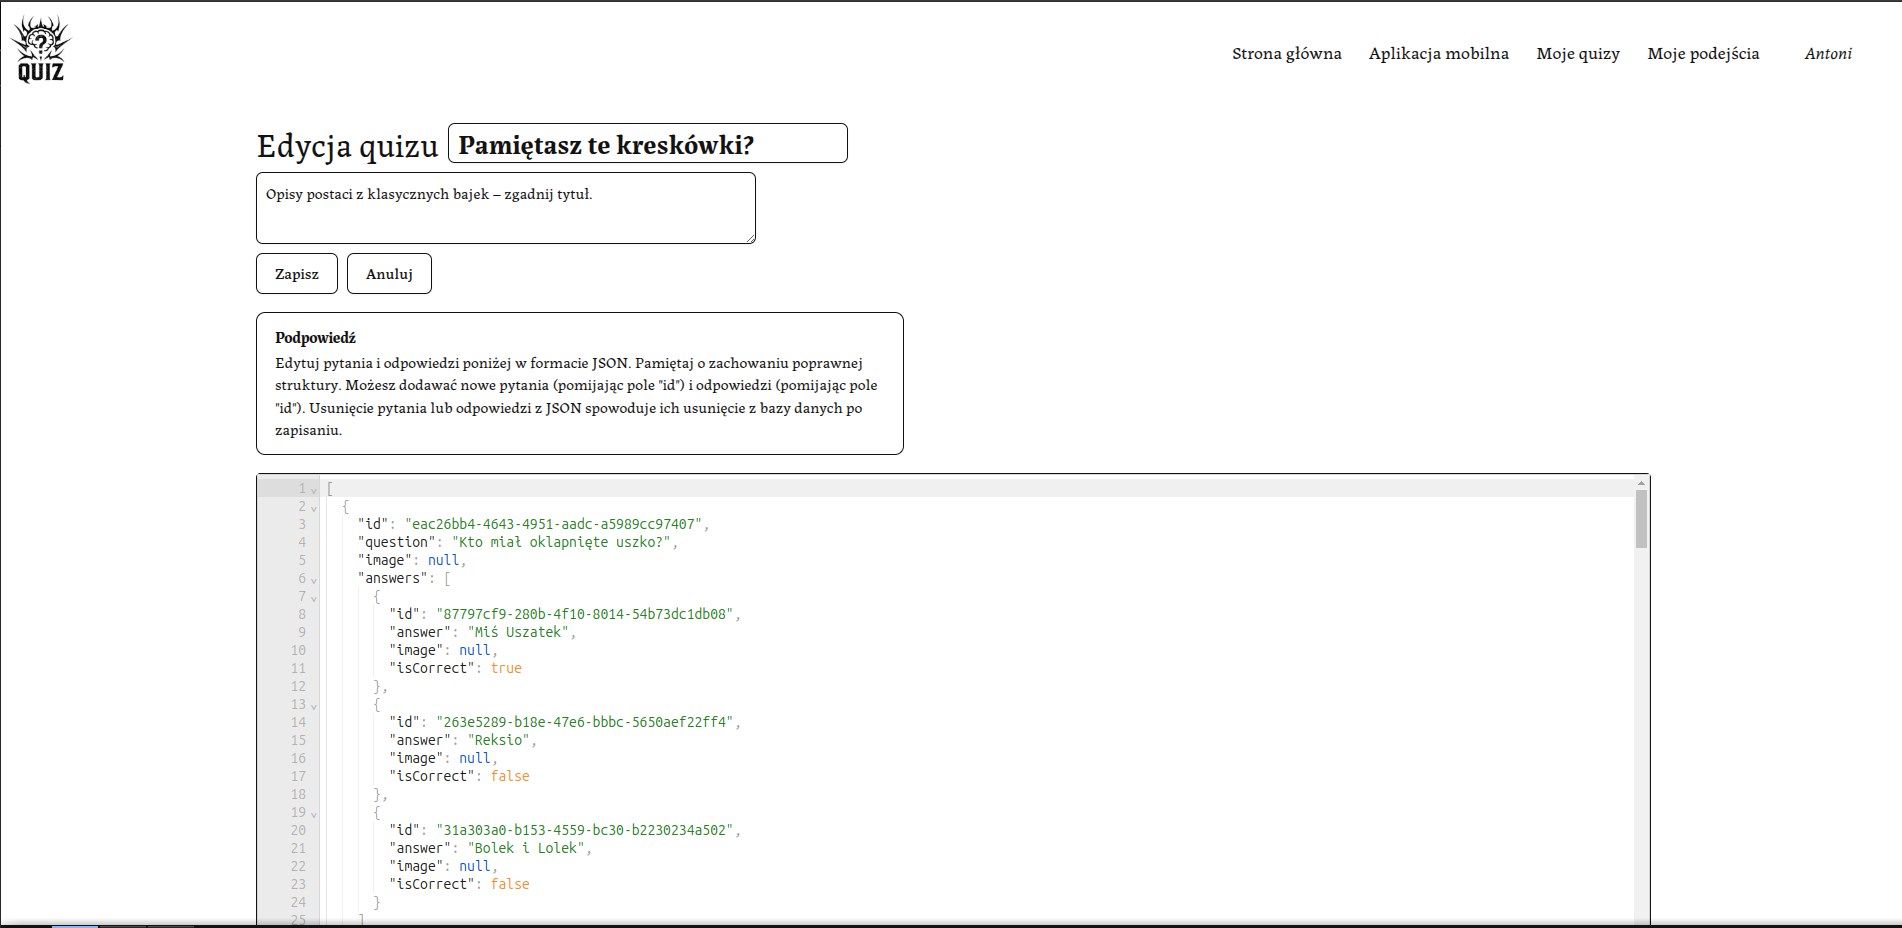
\includegraphics[width=0.5\textwidth]{../_assets/web/edit.png}
            \caption{Edytor quizu.}
            \label{fig:edit}
          \end{figure}
        \end{minipage}

		\item Lista quizów \\
        \begin{minipage}{0.4\textwidth}
          \begin{itemize}
            \item Możemy przeglądać listę quizów. Są tutaj widoczne nasze quizy i publiczne quizy innych użytkowników.
          \end{itemize}
        \end{minipage}
        \begin{minipage}{0.6\textwidth}
          \begin{figure}[H]
            \centering
            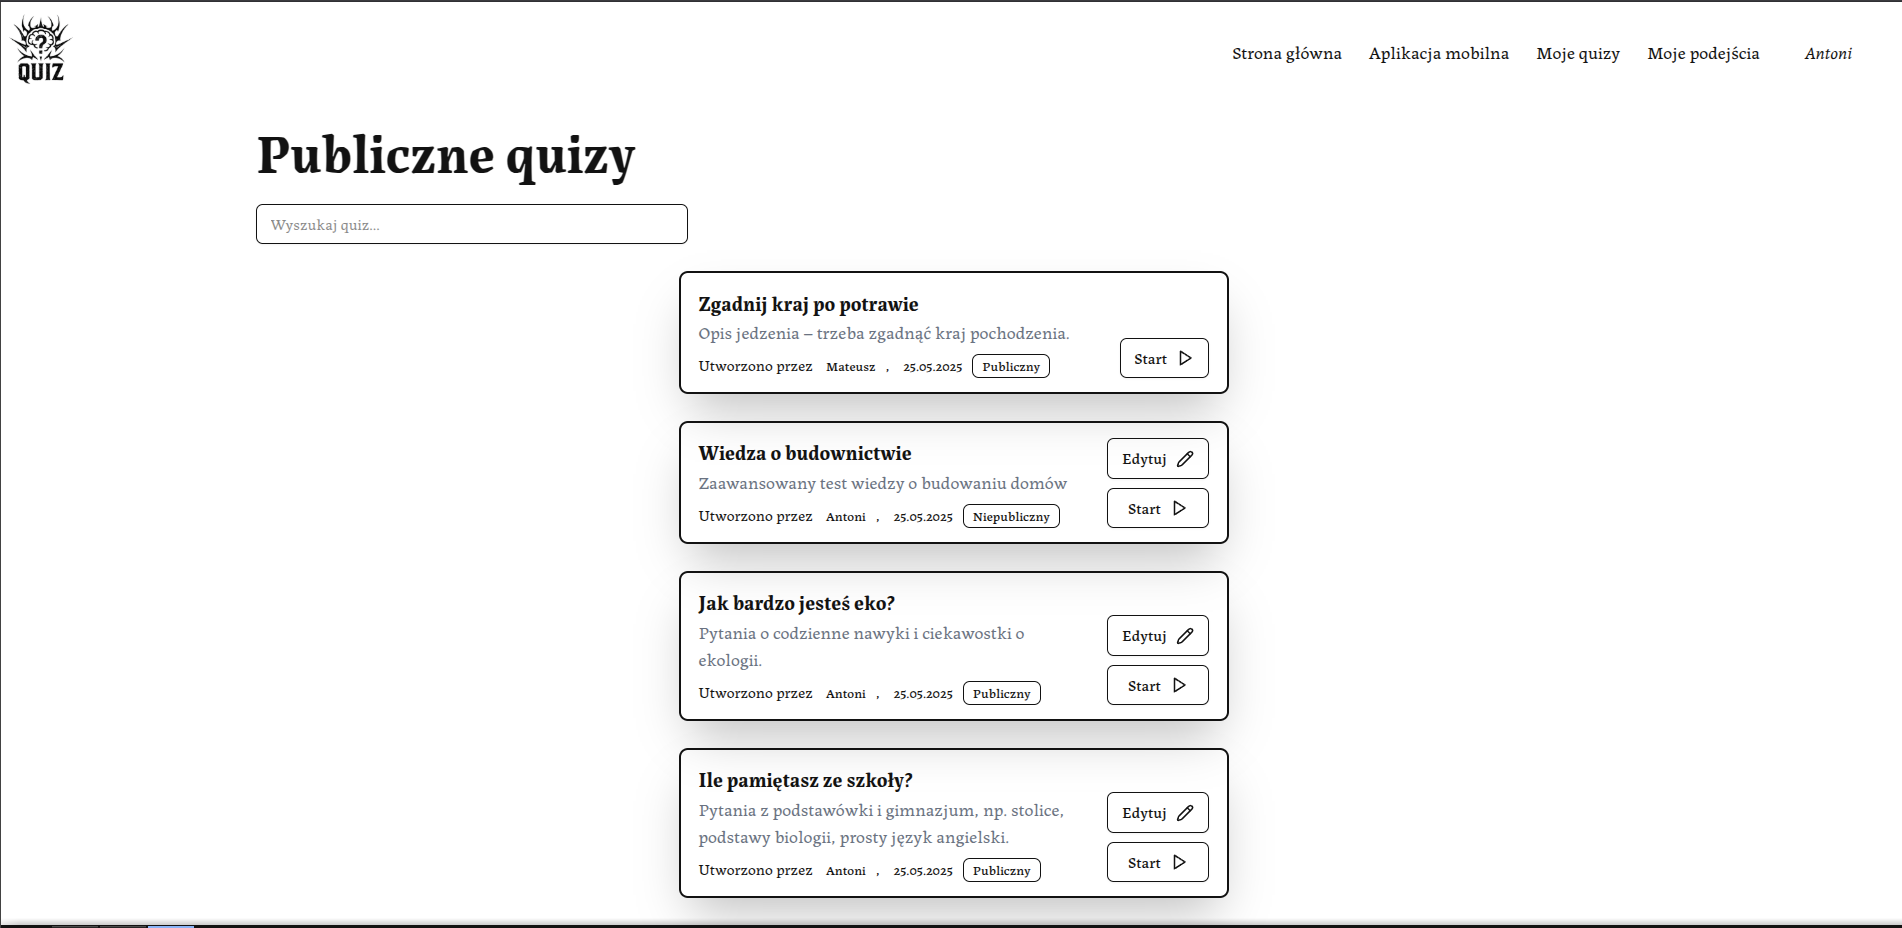
\includegraphics[width=0.5\textwidth]{../_assets/web/quizzes.png}
            \caption{Lista quizów (jest to też strona główna po zalogowaniu).}
            \label{fig:quizzes}
          \end{figure}
        \end{minipage}

		\item Podejście do quizu \\
        \begin{minipage}{0.4\textwidth}
          \begin{itemize}
            \item Rozpoczynając podejście wyświetlana jest lista pytań.
            \item Przy każdym pytaniu możemy sprawdzić poprawność odpowiedzi.
          \end{itemize}
        \end{minipage}
        \begin{minipage}{0.6\textwidth}
          \begin{figure}[H]
            \centering
            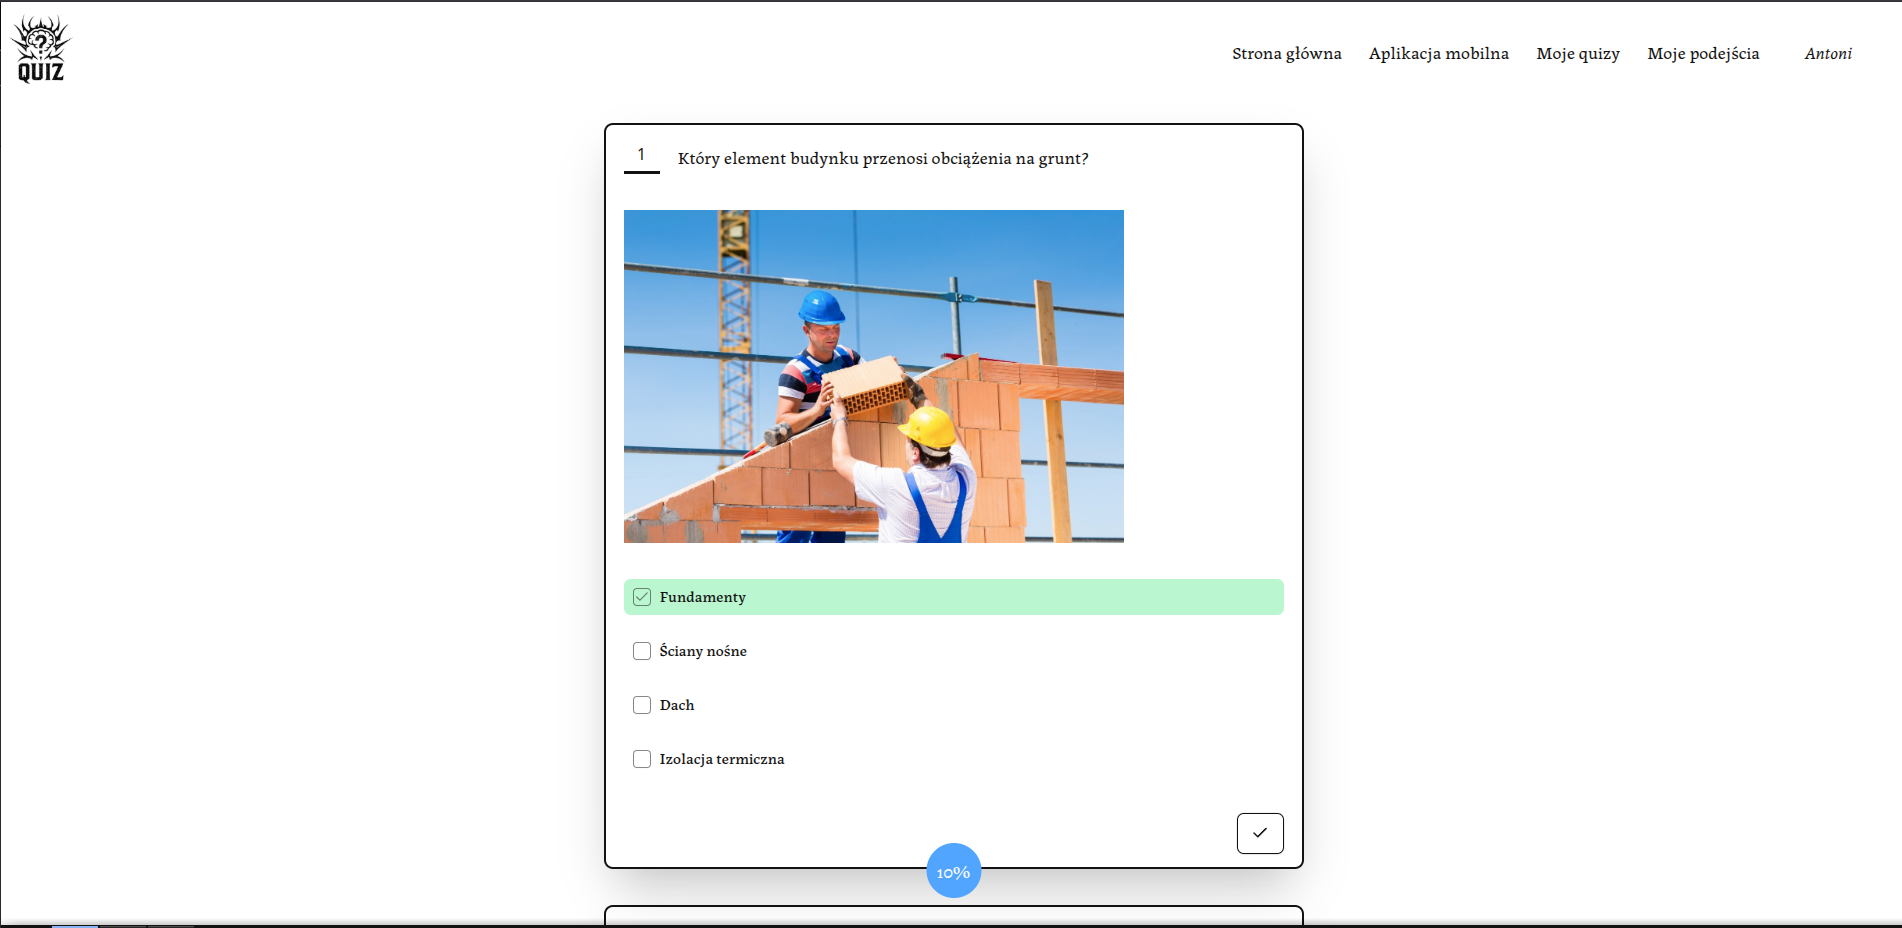
\includegraphics[width=0.5\textwidth]{../_assets/web/attempt.png}
            \caption{Podejście do quizu.}
            \label{fig:attempt}
          \end{figure}
        \end{minipage}

		\item Podsumowanie podejścia \\
        \begin{minipage}{0.4\textwidth}
          \begin{itemize}
            \item Przy każdym podejściu mamy możliwość sprawdzenia podsumowania.
            \item W podsumowaniu wyświetlane są podstawowe informacje o podejściu, takie jak czas trwania i liczba poprawnych odpowiedzi.
          \end{itemize}
        \end{minipage}
        \begin{minipage}{0.6\textwidth}
          \begin{figure}[H]
            \centering
            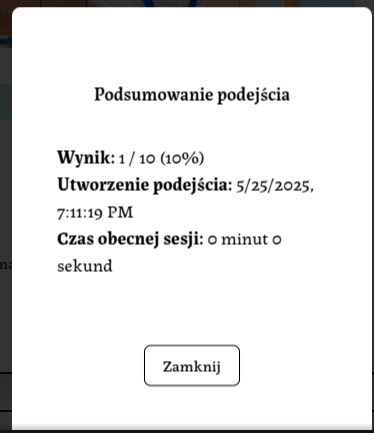
\includegraphics[width=0.5\textwidth]{../_assets/web/summary.png}
            \caption{Podsumowanie podejścia do quizu.}
            \label{fig:summary}
          \end{figure}
        \end{minipage}

      \end{enumerate}


    \section{Wnioski}
        Przed rozpoczęciem projektu miałem doświadczenie w tworzeniu aplikacji webowych w bibliotece React.
        Projekt ten pokazał mi, że współcześnie Vue jest koncepcyjnie bardzo podobne do Reacta, a różnice znajdują się głównie w sposobie zarządzania stanem i strukturze komponentów.
        Poszerzyłem wiedzę o frameworku Vue oraz o architekturze aplikacji opartych na GraphQL.

\end{document}